\section{Results and Discussion}\label{sec:results}

\subsection{Overview}
This section summarizes the empirical evidence that supports our pipeline choices and diagnoses remaining failure modes. 

Confidence intervals reported in descriptive tables use the normal approximation over per-query scores and are explicitly labeled as descriptive
summaries rather than inferential tests. They do not adjust for multiple comparisons. "nvidia/llama-nemotron-rerank-1b-v2" and "Nemotron" are used interchangeably.

Table~\ref{tab:main-results} reports representative runs spanning lexical tuning, hybrid retrieval and neural reranking. Values are rounded to three decimals. 

\begin{table*}[htbp]
    \centering
    \footnotesize
    \caption{Representative English run-analysis results performed on the English train dataset en\_train.json}\label{tab:main-results}
    \resizebox{\textwidth}{!}{%
    \begin{tabular}{p{4.0cm} p{7.6cm} c c}
        \toprule
        Run label & Key configuration & MRR@5 & Recall@100 \\
        \midrule
        Analyzer V1.12 & BM25 retrieval with 
        stopword removal (stoplist\_ebscohost\_medline\_cinahl.txt), trim filter, removal of the \# symbol, no removal of @, accent normalization (ASCIIFoldingFilter), LowerCaseFilter, EnglishPossessiveFilter, KstemFilter, no use of WordDelimitedGraphFilter, searcher with OR boolean queries and BAAI/bge-large-en-v1.5 query expansion, no rerank.
        & 0.450 & 0.783 
        \\
        Analyzer V2 & Differ from the Analyzer V1.12 simply for choosing a broader and more comprehensive stoplist (stoplist\_en\_ranksnl\_large.txt). & 0.503 & 0.796
        \\
        bge\_m3\_hybrid\_315 & BGE-M3 hybrid retrieval with dense, sparse, and ColBERT weights of $0.35$, $0.15$, and $0.50$. & 0.557 & 0.837 \\
        bge\_m3\_hybrid\_513 & BGE-M3 hybrid retrieval with dense, sparse, and ColBERT weights of $0.50$, $0.15$, and $0.35$. & 0.557 & 0.839 \\
        Nemotron top-100 & bge\_m3\_hybrid\_513 candidates reranked with nvidia/llama-nemotron-rerank-1b-v2 with depth k=100. & 0.685 & 0.839 \\
        Nemotron top-1000 & bge\_m3\_hybrid\_513 candidates reranked with nvidia/llama-nemotron-rerank-1b-v2 with depth k=1000. & 0.702 & 0.911 \\
        Qwen3-4B top-100 & bge\_m3\_hybrid\_513 candidates reranked with Qwen/Qwen3-reranker-4B with depth k=100. & 0.662 & 0.839 \\
        GTE-ModernBERT top-100 & bge\_m3\_hybrid\_513 candidates reranked with Alibaba-NLP/gte-reranker-modernbert-base with depth k=100. & 0.652 & 0.852 \\
        \bottomrule
    \end{tabular}%
    }
\end{table*}


\subsection{Runs comparison on the TRAIN English split}\label{sub:run-comparison}

Hybrid variants differ only in the linear combination of dense, sparse and ColBERT-style BGE-M3 signals. Here we provide a fuller representation more metrics-driven. We have abbreviated bge\_m3\_hybrid\_315's system to H315 (same convention for other hybrid-retrieval system), similar convention for Nemotron's systems (N), Qwen3-4B (Q) and gte-reranker-modernbert-base (GTE). 

\begin{table*}[htbp]
    \centering
    \footnotesize
    \caption{Run comparison on the en\_train.json file. $\Delta$ takes as reference the H513 run.}\label{tab:run-comparison}
    \resizebox{\textwidth}{!}{%
    \begin{tabular}{p{1cm} p{7.6cm} r r r r r}
        \toprule
        Run & Configuration & MRR@5 & Recall@100 & MAP & nDCG@10 & $\Delta$ MRR@5 \\
        \midrule
        H424 & BGE-M3 weights $0.40/0.20/0.40$ & 0.5067 & 0.8277 & 0.5201 & 0.5531 & -0.0500 \\
        H514 & BGE-M3 weights $0.50/0.10/0.40$ & 0.5141 & 0.8327 & 0.5273 & 0.5595 & -0.0426 \\
        H414 & BGE-M3 weights $0.45/0.10/0.45$ & 0.5171 & 0.8327 & 0.5302 & 0.5621 & -0.0396 \\
        \textbf{H513} & \textbf{BGE-M3 weights 0.50/0.15/0.35} & \textbf{0.5567} & \textbf{0.8392} & \textbf{0.5688} & \textbf{0.5956} & \textbf{0.0000} \\
        H315 & BGE-M3 weights $0.35/0.15/0.50$ & 0.5572 & 0.8365 & 0.5692 & 0.5957 & +0.0005 \\
        Q100 & H513 candidates reranked with Qwen3-4B, top-100 retained & 0.6624 & 0.8392 & 0.6696 & 0.6953 & +0.1057 \\
        GTE100 & H513 candidates reranked with gte-reranker-modernbert-base, top-100 retained & 0.6511 & 0.8392 & 0.6594 & 0.6830 & +0.0944 \\
        N100 & H513 candidates reranked with Nemotron, top-100 retained & 0.6847 & 0.8392 & 0.6909 & 0.7146 & +0.1280 \\
        N500 & H513 candidates reranked with Nemotron, top-500 retained & 0.7010 & 0.8986 & 0.7096 & 0.7342 & +0.1443 \\
        \textbf{N1000} & \textbf{H513 candidates reranked with Nemotron, top-1000 retained} & \textbf{0.7018} & \textbf{0.9109} & \textbf{0.7111} & \textbf{0.7357} & \textbf{+0.1451} \\
        \bottomrule
    \end{tabular}%
    }
\end{table*}

H424 is the weakest reported hybrid configuration while H513 and H315 perform substantially better on early-precision metrics. H513 has an advantage in Recall@100 relative to H315, which motivates its selection as the candidate generator for the full pipeline: retrieval should prioritize coverage that the reranker can refine. Neural reranking (Nemotron) yields the largest improvements: moving from H513 to N1000 increases MRR@5 by roughly 0.145 and increases Recall@100 notably, showing that deeper reranking improves both precision and coverage. However, gains in MRR@5 beyond top-500 are marginal, suggesting diminishing returns for very deep pools.

As shown later in Section~\ref{sub:statistical-analysis}, formal non-parametric inference supports these conclusions: the Friedman omnibus rejects equality across systems and Holm-corrected pairwise Wilcoxon tests identify the same stage-aligned differences summarized in Table~\ref{tab:stage-specific-tests}.

\subsection{Multilingual DEV split validation}\label{sub:multilingual-dev}

DEV runs were not used to re-tune the TRAIN analysis pipelines. They are presented as external validation with appropriately wider uncertainty bands.

\begin{table*}[htbp]
    \centering
    \footnotesize
    \caption{Fine-tuned Nemotron LoRA validation on labeled development data. The final column reports rank-bucket counts for strong successes and unresolved failures.}\label{tab:multilingual-dev}
    \resizebox{\textwidth}{!}{%
    \begin{tabular}{l r r r r r r r}
        \toprule
        Split & Queries & MRR@5 & 95\% CI & Recall@100 & MAP & nDCG@10 & Rank 1 / Missing \\
        \midrule
        EN DEV & 3905 & 0.7160 & [0.7030, 0.7290] & 0.9129 & 0.7243 & 0.7483 & 2574 / 241 \\
        FR DEV & 702  & 0.7599 & [0.7310, 0.7888] & 0.9288 & 0.7672 & 0.7894 & 496 / 40 \\
        DE DEV & 386  & 0.6736 & [0.6305, 0.7168] & 0.8860 & 0.6820 & 0.7080 & 237 / 29 \\
        \bottomrule
    \end{tabular}%
    }
\end{table*}

The development results suggest that the final pipeline generalizes reasonably well across languages after translation but not uniformly. French is the strongest development split with MRR@5 of 0.7599 and Recall@100 of 0.9288. German is the weakest with MRR@5 of 0.6736 and the widest confidence interval.
Rank-bucket counts corroborate these summaries: French has the largest fraction of rank-1 successes and the fewest missing cases (496/40), while German shows fewer rank-1 hits and a higher unresolved fraction relative to its query count (237/29).
In practice this pattern suggests that the reranker generalizes well to translated queries in French, English remains competitive and that German's lower point estimates and wider intervals are plausibly driven by both smaller sample size and translation/terminology drift. These DEV findings validate the pipeline qualitatively and motivated the decision to use a deeper top-2000 pool in the final TEST submission to favour recall.

\subsection{Experimental Results on the TEST Set}
As can be seen in Table \ref{tab:TEST-run-comparison}, all the previous ideas and assumptions have been confirmed in the TEST set. Increasing the depth of the reranking, managing metadata such as authors, fine-tuning, and selecting the reranker led to results that allowed us to finish fifth in the rankings, despite having limited hardware. Qwen/Qwen3-Reranker-4B seems to have difficulties to correctly interpret additional information such as authors and this may be due to its nature as an LLM-based reranker, whereas other cross-encoders perform better.

\begin{table*}[htbp]
    \centering
    \footnotesize
    \caption{Runs comparison on the final\_en\_test.json set. They are all based on bi513\_encoder\_results\_bge\_large\_topk1000, FT stands for fine-tuned.}\label{tab:TEST-run-comparison}
    \resizebox{\textwidth}{!}{%
    \begin{tabular}{l r r r r r r}
        \toprule
        Run & MRR@5 & F1@1 & MAP & nDCG@5 & Recall@100 \\
        \midrule
        \textbf{nemotronFT\_topk2000\_withAuthors} & \textbf{0.7117} & \textbf{0.6501} & \textbf{0.7202} & \textbf{0.7346} & \textbf{0.9235} \\
        nemotronFT\_topk100\_withAuthors & 0.6918 & 0.6358 & 0.6972 & 0.7118 & 0.8371 \\
        nemotron\_topk100\_withAuthors & 0.6782 & 0.6229 & 0.6845 & 0.6982 & 0.8371 \\
        nemotron\_topk100\_noAuthors & 0.6647 & 0.6058 & 0.6721 & 0.6858 & 0.8371 \\
        Qwen3-Reranker-4B\_topk100\_noAuthors & 0.6421 & 0.5810 & 0.6505 & 0.6644 & 0.8371 \\
        gte\_modernbert\_topk100\_withAuthors & 0.6382 & 0.5841 & 0.6467 & 0.6588 & 0.8371 \\
        Qwen3-Reranker-4B\_topk100\_withAuthors & 0.6337 & 0.5734 & 0.6430 & 0.6556 & 0.8371 \\
        gte\_modernbert\_topk100\_noAuthors & 0.6304 & 0.5757 & 0.6395 & 0.6507 & 0.8371 \\
        bi513\_encoder\_results\_bge\_large\_topk1000 & 0.5047 & 0.4378 & 0.5195 & 0.5308 & 0.8371 \\
        bi414\_encoder\_results\_bge\_large\_topk1000 & 0.5035 & 0.4371 & 0.5181 & 0.5297 & 0.8348 \\
        \bottomrule
    \end{tabular}%
    }
\end{table*}

\subsubsection{Official TEST set submission}\label{sub:test-results}

The submitted systems use the same four-stage pipeline described in Section~\ref{sec:methodology}: translate non-English queries into English, expand the query, retrieve candidates with BGE-M3 hybrid retrieval and rerank with the fine-tuned Nemotron LoRA cross-encoder.

\begin{table}[htbp]
    \centering
    \footnotesize
    \caption{Official TEST set results metrics. The aggregate row is a micro-average over all queries.}\label{tab:test-effectiveness}
    \begin{tabular}{l c c c c}
        \toprule
        Language & MRR@5 & Recall@100 & MAP & nDCG@10 \\
        \midrule
        EN & 0.7117 & 0.9235 & 0.7202 & 0.7469 \\
        FR & 0.7400 & 0.9328 & 0.7479 & 0.7689 \\
        DE & 0.6806 & 0.9155 & 0.6907 & 0.7213 \\
        Aggregate & 0.7126 & 0.9240 & 0.7212 & 0.7474 \\
        \bottomrule
    \end{tabular}
\end{table}

Table~\ref{tab:test-effectiveness} reports micro-averaged metrics per language. TEST metrics confirm the DEV pattern: French shows the highest aggregate MRR@5, English is competitive, and German shows lower scores and larger uncertainty. For the TEST submission we used a deeper reranking pool (top-2000) to favor recall for the final delivered runs. DEV experiments indicated modest but consistent recall gains when increasing the pool depth, so we opted for a deeper pool in TEST to maximize coverage of the gold document.

\subsection{Statistical analysis}\label{sub:statistical-analysis}

We separate descriptive summaries from formal hypothesis tests. Descriptive confidence intervals (Figure~\ref{fig:mrr-mean-ci}) summarize uncertainty around mean per-query scores but do not by themselves imply statistical significance and do not correct for multiple comparisons. For inference we follow a stage-aligned strategy: test retrieval-stage decisions on Recall@100 (coverage), and test reranking-stage decisions on MRR@5 (early precision). Because per-query metrics are bounded and strongly non-normal, we use the non-parametric Friedman repeated-measures test as the omnibus alternative to a repeated-measures ANOVA. For each metric we perform a Friedman omnibus test over repeated measures: when the omnibus rejects, we report pairwise Wilcoxon signed-rank tests with Holm correction to control family-wise error across all tested pairs~\cite{Friedman1937,Wilcoxon1945}.

\subsubsection{Descriptive statistics}

Table~\ref{tab:mrr-descriptive-stats} summarizes per-query MRR@5 for H513 and Nemotron reranking depths on the TRAIN split. Reranking shifts the entire distribution: the median increases from 0.5 (H513) to 1.0 for Nemotron runs and the first quartile rises from 0.0 to 0.25, indicating that a substantially larger fraction of queries receive a non-zero early-precision score after reranking.

\begin{table*}[htbp]
    \centering
    \footnotesize
    \caption{Descriptive statistics of per-query MRR@5 on the TRAIN English split. Confidence intervals use the normal approximation over queries.}\label{tab:mrr-descriptive-stats}
    
    \begin{tabular}{l r r r r r r r r}
        \toprule
        Run & Mean & Median & Std. dev. & Variance & Q1 & Q3 & 95\% CI \\
        \midrule
        H513  & 0.5567 & 0.5 & 0.4614 & 0.2129 & 0.00 & 1.00 & [0.5493, 0.5641] \\
        N100  & 0.6847 & 1.0 & 0.4303 & 0.1852 & 0.25 & 1.00 & [0.6778, 0.6916] \\
        N500  & 0.7010 & 1.0 & 0.4229 & 0.1788 & 0.25 & 1.00 & [0.6943, 0.7078] \\
        N1000 & 0.7018 & 1.0 & 0.4223 & 0.1784 & 0.25 & 1.00 & [0.6950, 0.7086] \\
        \bottomrule
    \end{tabular}%
\end{table*}

\begin{figure*}[htbp]
    \centering
    \begin{subfigure}[t]{0.49\textwidth}
        \centering
        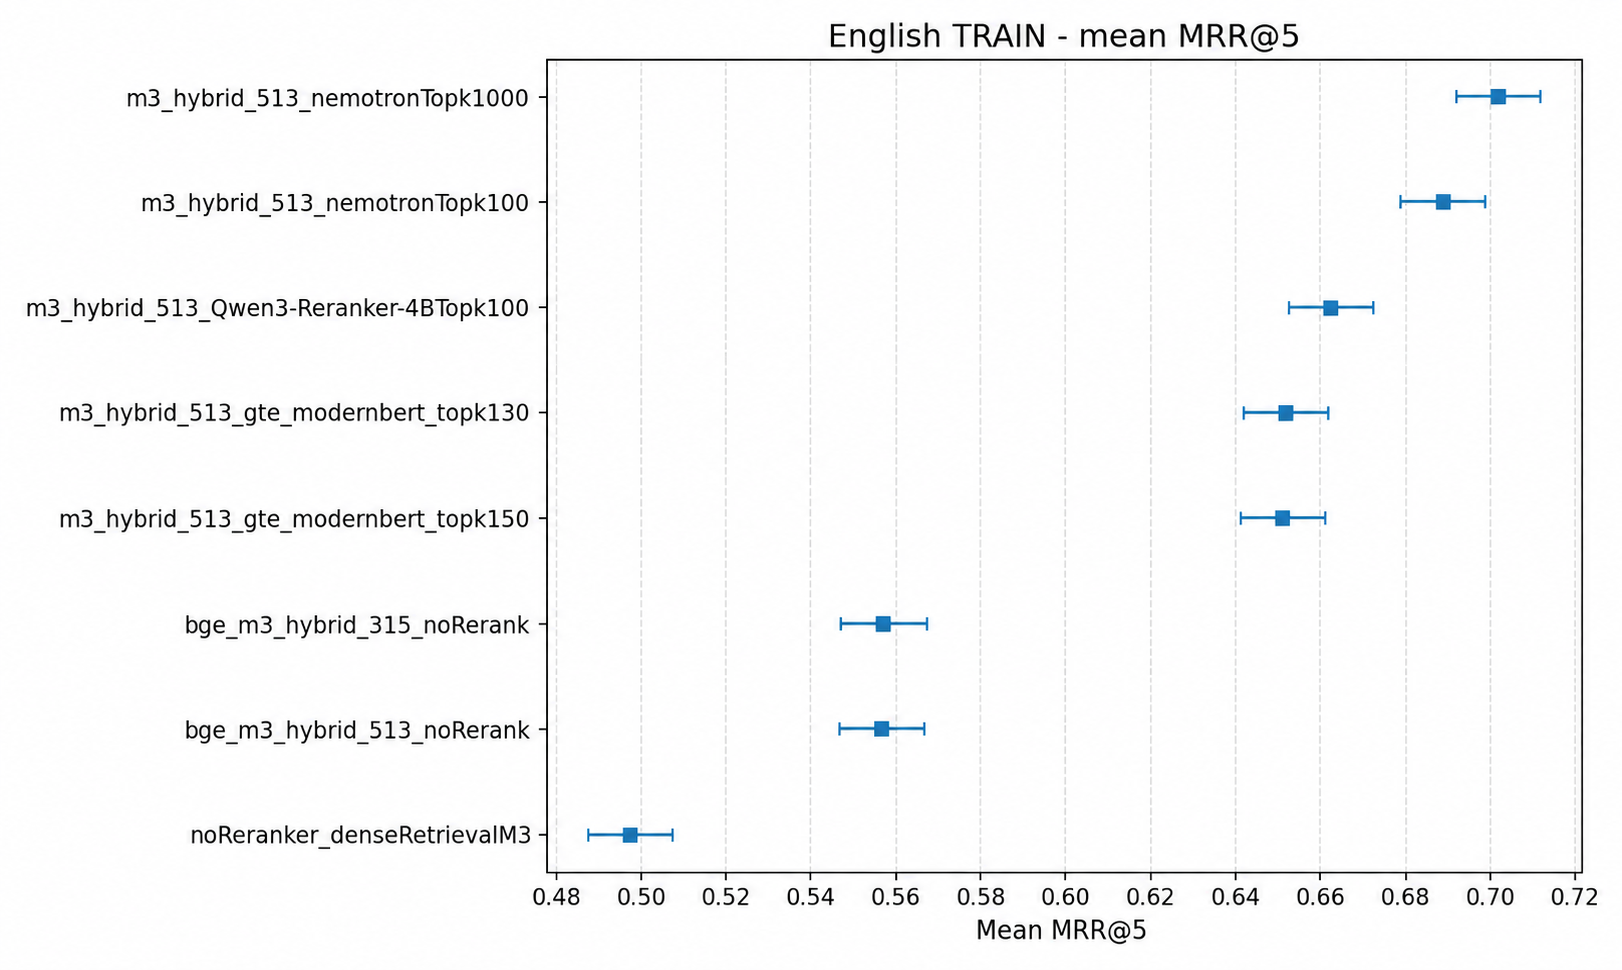
\includegraphics[width=\linewidth]{../figure/MRR5_TRAIN.png}
        \caption{English TRAIN.}
    \end{subfigure}
    \hfill
    \begin{subfigure}[t]{0.49\textwidth}
        \centering
        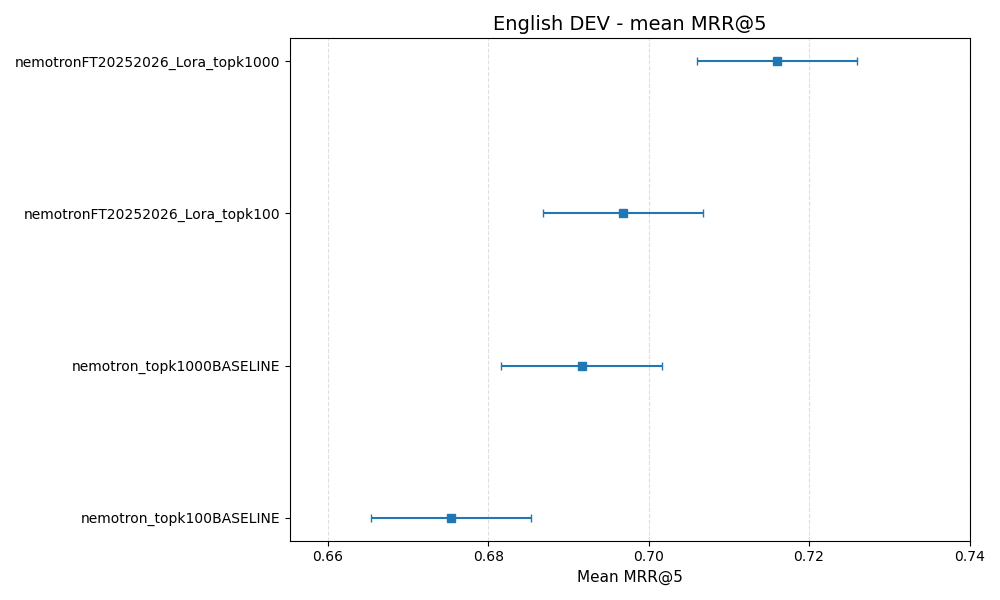
\includegraphics[width=\linewidth]{../figure/MRR5_DEV.png}
        \caption{English DEV.}
    \end{subfigure}
    \caption{Mean MRR@5 with normal-approximation 95\% confidence intervals for the English TRAIN and DEV statistical-analysis runs. These bands are descriptive only and do not account for multiple comparisons.}\label{fig:mrr-mean-ci}
\end{figure*}

Figure~\ref{fig:mrr-mean-ci} visualizes the mean per-query MRR@5 and the associated normal-approximation 95\% confidence intervals for both the large TRAIN split and the smaller DEV split. The plot makes two descriptive points clear:
\begin{itemize}
    \item Nemotron reranked systems lie well above the retained hybrid baselines on mean MRR@5;
    \item The TRAIN CIs are much narrower than DEV's (owing to its larger sample), which increases confidence in the descriptive means reported in Table~\ref{tab:mrr-descriptive-stats}.
\end{itemize}

These CIs are descriptive uncertainty bands (normal-approximation). Formal hypothesis tests are reported in the following sections.

\subsubsection{Formal significance testing}

The Friedman omnibus test rejects the null hypothesis that all English TRAIN systems share the same per-query MRR@5 distribution ($\chi^2=21368.46$, $p<0.001$). We then report two-sided Wilcoxon signed-rank tests with Holm correction to control the family-wise error rate across all pairwise system comparisons for each metric. Table~\ref{tab:formal-statistical-tests} shows the comparisons most relevant to pipeline decisions. Because of our staged pipeline, MRR@5 is the primary inferential target for reranking-stage comparisons, while Recall@100 is used for retrieval-stage comparisons.

\begin{table*}[htbp]
    \centering
    \footnotesize
    \caption{Formal statistical tests on per-query MRR@5 for the English TRAIN split. The Friedman row is the omnibus test over all tested systems and 14,977 queries; pairwise rows use two-sided Wilcoxon signed-rank tests with Holm correction over all pairwise comparisons. Pairwise mean differences are computed as the second system minus the first.}\label{tab:formal-statistical-tests}
    \resizebox{\textwidth}{!}{%
    \begin{tabular}{l p{4.1cm} r r l}
        \toprule
        Test & Systems / comparison & Mean difference & $p_{\mathrm{holm}}$ & Interpretation \\
        \midrule
        Friedman omnibus & All tested English TRAIN systems & -- & $<0.001$ & At least one system differs \\
        Wilcoxon--Holm & H315 vs H513 & -0.0005 & 1.0000 & No significant difference \\
        Wilcoxon--Holm & H424 vs H513 & +0.0500 & $8.58\times10^{-116}$ & H513 significantly better \\
        Wilcoxon--Holm & H513 vs N1000 & +0.1451 & $<0.001$ & N1000 significantly better \\
        Wilcoxon--Holm & N1000 vs N500 & -0.0008 & 0.0497 & Significant but negligible in size \\
        \bottomrule
    \end{tabular}%
    }
\end{table*}

The inference supports two practical conclusions. First, H513 and H315 are indistinguishable on MRR@5: choose between them using retrieval-stage diagnostics (Recall@100) and operational constraints. Second, the Nemotron reranker produces a large and statistically supported gain over the retained hybrid baseline. The small difference between N500 and N1000 is statistically detectable after Holm correction but practically negligible in MRR@5, suggesting practitioners may prefer N500 when latency or cost is a concern.

\subsubsection{Stage-specific tests}

To align inference with pipeline objectives we repeat Holm-corrected pairwise tests on Recall@100 for retrieval-stage comparisons and on MRR@5 for reranking-stage comparisons. Table~\ref{tab:stage-specific-tests} summarizes the comparisons that most directly motivated our pipeline choices.

\begin{table*}[htbp]
    \centering
    \footnotesize
    \caption{Holm-corrected pairwise tests aligned with the pipeline objective. For retrieval-stage comparisons, $\Delta$ is the preferred hybrid minus the comparator on Recall@100. For reranking-stage comparisons, $\Delta$ is N1000 minus the comparator on MRR@5.}
    \label{tab:stage-specific-tests}
    \resizebox{\textwidth}{!}{%
    \begin{tabular}{l p{4.0cm} r r l}
        \toprule
        Stage & Comparison & $\Delta$ & $p_{\mathrm{holm}}$ & Conclusion \\
        \midrule
        Retrieval & H513 vs H315 & +0.0026 & 0.0007 & H513 better on Recall@100 \\
        Retrieval & H513 vs H414 & +0.0065 & 0.0027 & H513 better on Recall@100 \\
        Retrieval & H513 vs H424 & +0.0115 & $7.81\times10^{-9}$ & H513 better on Recall@100 \\
        Retrieval & H513 vs H514 & +0.0065 & 0.0027 & H513 better on Recall@100 \\
        \midrule
        Reranking & N1000 vs H513 & +0.1451 & $<0.001$ & N1000 better on MRR@5 \\
        Reranking & N1000 vs N500 & +0.0008 & 0.0497 & detectable but negligible \\
        \bottomrule
    \end{tabular}%
    }
\end{table*}

Together these tests support our pipeline choices. H513 is the best-supported hybrid candidate generator on Recall@100, and N1000 yields the largest early-precision gains on MRR@5. The incremental MRR@5 gain from N500 to N1000 is statistically detectable but practically tiny, which implies an operational trade-off between latency and marginal accuracy.

\subsubsection{Rank-bucket and error analysis}

Table~\ref{tab:rank-bucket-analysis} reports the rank position of the gold document for the retained hybrid and reranked runs. The analysis separates three qualitatively different error types. A gold paper is counted as \textit{missing} only when its gold \texttt{pubkey} is absent from every document available in the ranked file for that query. Thus, for runs with retained deep candidate lists, missing cases indicate that the reranker cannot recover the document from its input pool. For runs available only as submitted top-100 lists, missing means absent from the available top-100 file and not necessarily absent from the original upstream retrieval pool.

\begin{table*}[htbp]
    \centering
    \footnotesize
    \caption{Rank buckets for the retained hybrid and reranked English runs. Percentages are computed within each split: 14,977 labeled English queries, 3,905 English DEV queries, and 6,076 English TEST queries.}
    \label{tab:rank-bucket-analysis}
    \resizebox{\textwidth}{!}{%
    \begin{tabular}{l l r r r r r r r}
        \toprule
        Split & Run & Queries & Rank 1 & Ranks 2--5 & Ranks 6--10 & Ranks 11--100 & Rank $>100$ & Missing \\
        \midrule
        EN TRAIN & H513 (topk100)
        & 14977
        & 7459 (49.8\%)
        & 2280 (15.2\%)
        & 715 (4.8\%)
        & 2114 (14.1\%)
        & 0 (0.0\%)
        & 2409 (16.1\%) \\
        EN TRAIN & N1000
        & 14977
        & 9697 (64.7\%)
        & 2057 (13.7\%)
        & 598 (4.0\%)
        & 1291 (8.6\%)
        & 405 (2.7\%)
        & 929 (6.2\%) \\
        EN DEV & N1000 FT
        & 3905
        & 2574 (65.9\%)
        & 538 (13.8\%)
        & 144 (3.7\%)
        & 309 (7.9\%)
        & 99 (2.5\%)
        & 241 (6.2\%) \\
        EN TEST & N100 FT
        & 6076
        & 3863 (63.6\%)
        & 821 (13.5\%)
        & 157 (2.6\%)
        & 245 (4.0\%)
        & 0 (0.0\%)
        & 990 (16.3\%)\\
        EN TEST & N2000 FT
        & 6076
        & 3950 (65.0\%)
        & 926 (15.2\%)
        & 229 (3.8\%)
        & 506 (8.3\%)
        & 0 (0.0\%)
        & 465 (7.7\%) \\
        \bottomrule
    \end{tabular}%
    }
\end{table*}

The labeled English comparison shows that the main effect of reranking is to move correct papers to the very top of the list. The best reranked run on the TRAIN split places the gold paper at rank 1 for 9697 queries, compared with 7459 for the retained hybrid single-stage run. It also reduces missing cases from 2409 to 929. The remaining errors are informative: for Nemotron Baseline, 1291 queries have the gold paper in ranks 11--100, indicating ranking failures rather than retrieval failures, whereas 929 queries remain missing from the available reranking pool and therefore cannot be recovered by the reranker.

The final English DEV and TEST runs follow the same pattern. Nemotron LoRA fine-tuned places the gold paper at rank 1 for 2574 of 3905 queries, and does so also for the TEST set with 3950 of 6076 queries. Their top-5 coverage is similar, with 3112 DEV queries and 4876 TEST queries resolved within the first five ranks. The DEV file contains 1000 ranked documents for each query, so the 99 cases in Rank $>100$ correspond to gold papers found by the retained reranking pool but not placed within the first 100 positions. Due to a problem at our main computer the TEST file used to compute the metrics contains only the submitted top-100 documents per query even though the calculation was performed with depth=2000. Consequently, Rank $>100$ is zero by construction and the 465 missing TEST cases should be interpreted as missing from the available submitted run rather than as evidence that the original upstream retrieval pool never retrieved the gold paper. The run N100 FT should help the reader to understand the improvement that the additional depth bring.


Overall, the bucket analysis indicates that reranking substantially improves early precision while leaving two residual failure modes. The first consists of ranking failures, where the gold paper is present but remains below the top-5 cutoff. The second consists of missing cases, which are more severe because they cannot be repaired by reranking alone. These missing cases are likely associated with severe vocabulary mismatch, translation drift, or claims whose wording emphasizes entities and contextual cues that are weakly represented in titles and abstracts.

Taken together, the Results section should be read as a labeled-split evaluation plus submission diagnostics rather than a complete official TEST effectiveness report. Our strongest conclusions are those directly supported by per-query gold labels and formal inference (paired Wilcoxon tests with Holm correction) on the TRAIN and DEV splits. 


\subsubsection{Error patterns and failure analysis}

Manual inspection of missing and low-ranked cases suggests several recurring failure modes:

\begin{enumerate}
    \item \textbf{Claim-to-metadata specificity mismatch:} claims that emphasize fine-grained experimental results, numeric outcomes, or methods not reflected in titles/abstracts are hard for the retriever to match.

    \item \textbf{Translation artifacts in non-English queries:} literal or imperfect translations introduce term shifts that reduce lexical overlap and semantic alignment with the English corpus.

    \item \textbf{Implicit references with little lexical overlap:} queries phrased as vague or conversational references ("this study") lack the lexical anchors that support retrieval, requiring stronger semantic modeling or additional context.
\end{enumerate}

\subsubsection{Performance by query characteristics}

Figure~\ref{fig:query-characteristics-mrr} reports a query-level characterization of the N1000 run on the English TRAIN split. Contrary to our initial intuition, token length alone is not positively associated with higher MRR@5. In this run, short queries with at most 20 tokens reach 0.760 MRR@5, medium-length queries reach 0.713, and long queries with at least 35 tokens reach 0.672. This suggests that longer tweet-like claims often add conversational or contextual material that does not necessarily help identify the target paper.

The named-entity cue analysis is more consistent with the retrieval intuition. Using a lightweight heuristic based on author-like capitalization patterns, acronyms, and institution or venue keywords, entity-rich queries reach 0.733 MRR@5, while entity-sparse queries reach 0.664. These observations remain exploratory and should be interpreted as heuristic patterns rather than formal statistical findings, but they support the value of hybrid retrieval that combines lexical anchors with semantic matching.

\begin{figure*}[htbp]
    \centering
    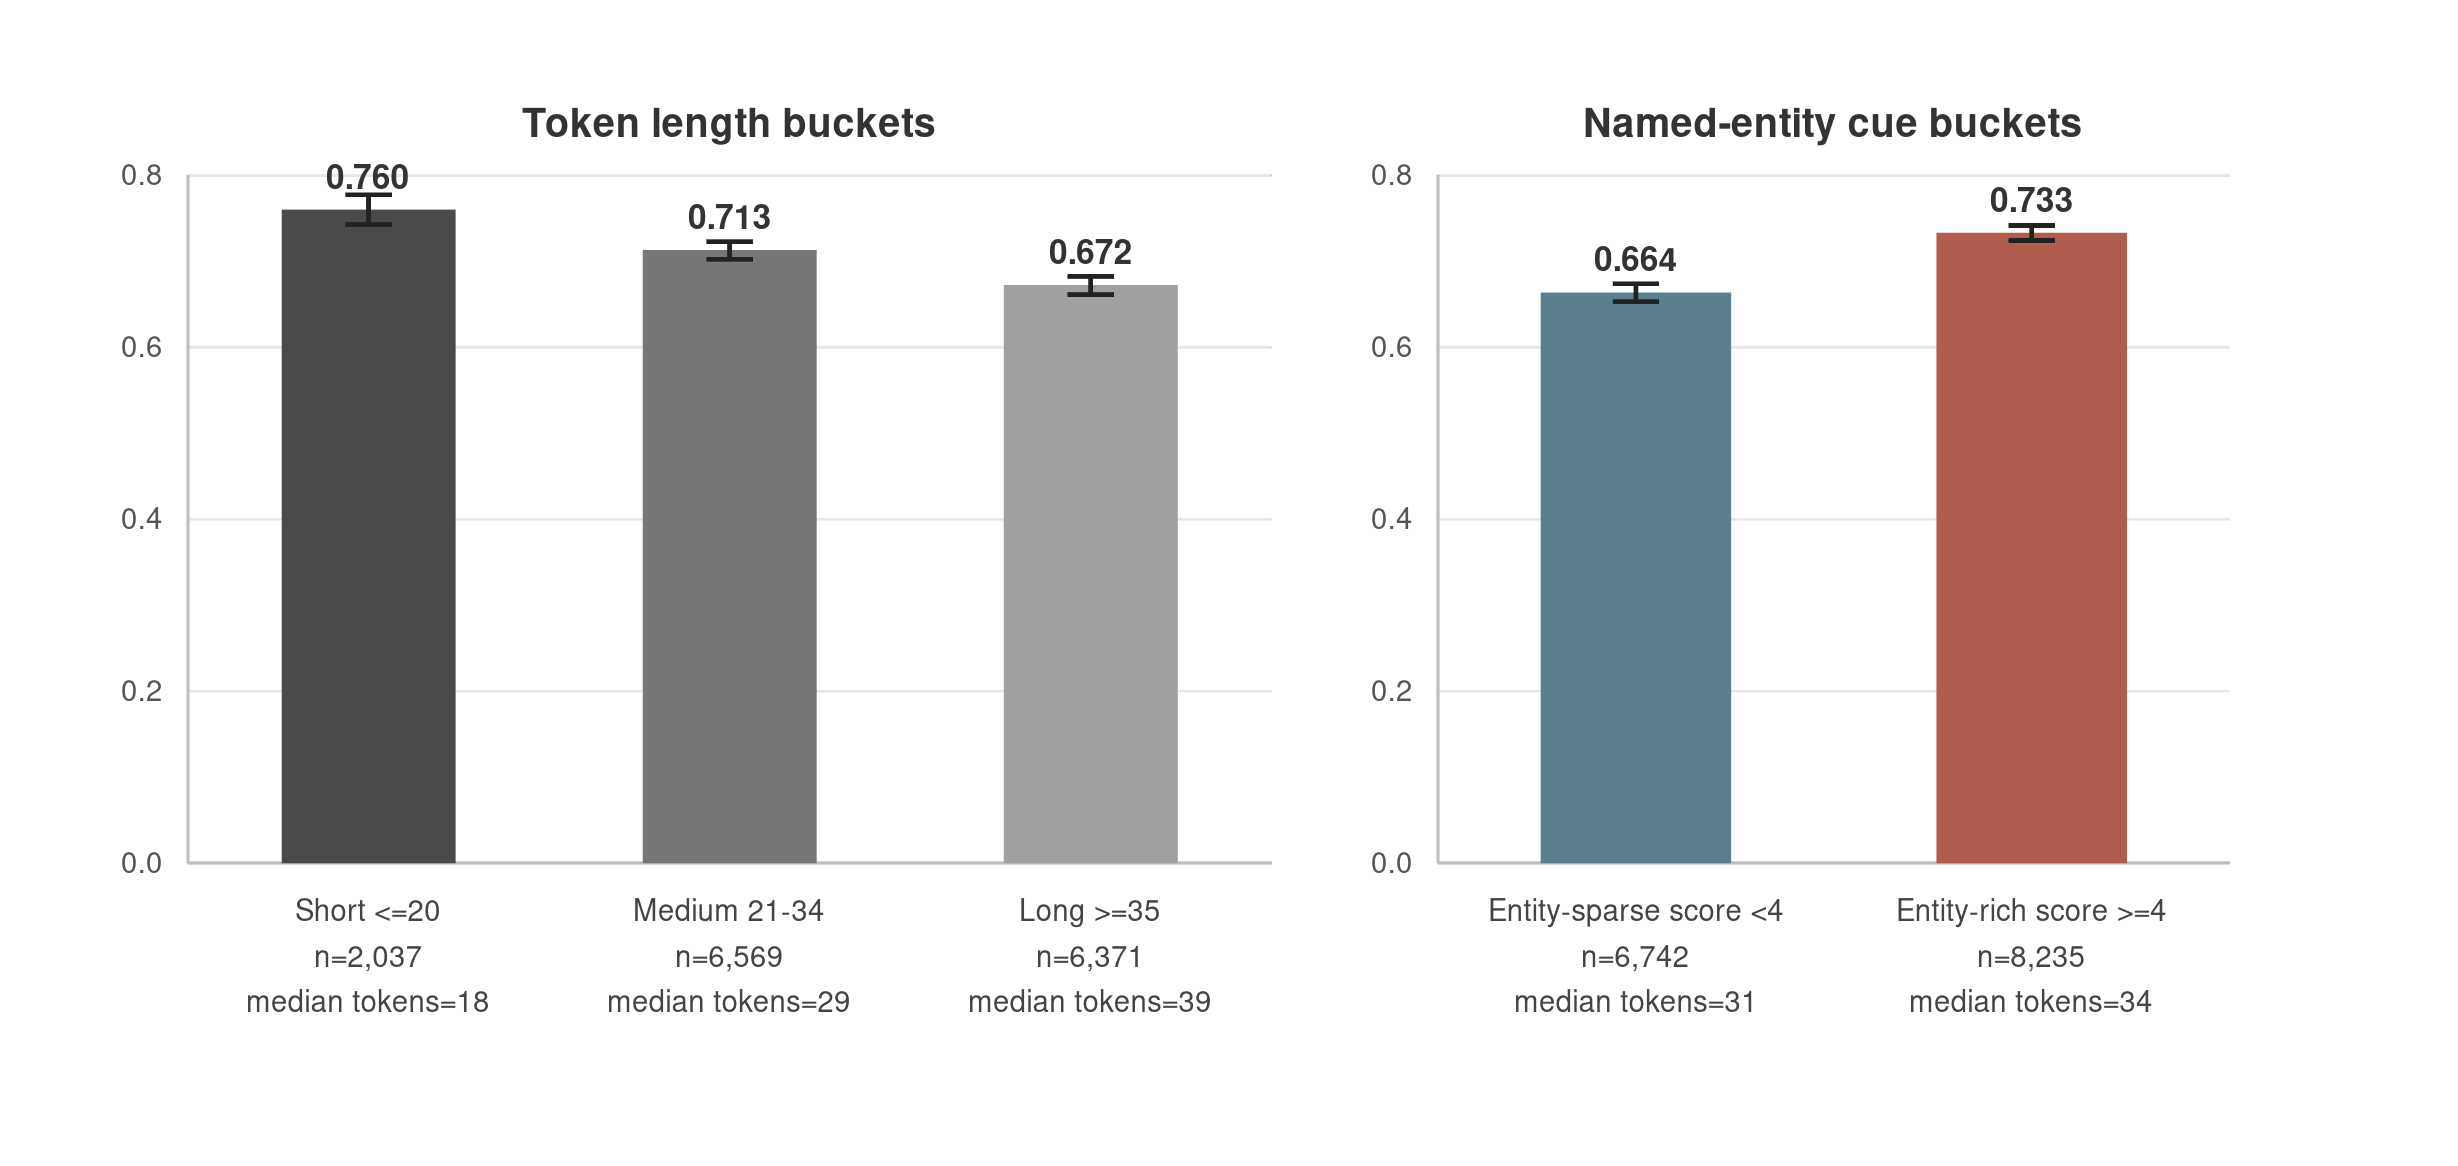
\includegraphics[width=0.95\textwidth]{../figure/query_characteristics_mrr.png}
    \caption{Mean per-query MRR@5 for the Nemotron Baseline English TRAIN run grouped by query length and by a lightweight named-entity cue score. Error bars show normal-approximation 95\% confidence intervals over queries.}\label{fig:query-characteristics-mrr}
\end{figure*}

\subsection{Reproducibility and summary}
In the repository \textit{https://bitbucket.org/upd-dei-stud-prj/seupd2526-retrix/src/master/} are stored almost all the runs (something exceeded the 100MB limit of the platform), scripts and programs used in the project.

In summary: combining descriptive summaries, stage-aligned formal inference, and rank-bucket diagnostics yields a coherent picture: H513 is the most defensible hybrid candidate generator on Recall@100, and Nemotron reranking (especially N1000) provides large, statistically supported gains in early precision (MRR@5). Remaining errors split between retrievable but low-ranked cases and true retrieval misses. Addressing the latter requires improved candidate coverage or query reformulation.